\documentclass[11pt,ignorenonframetext,]{beamer}
\setbeamertemplate{caption}[numbered]
\setbeamertemplate{caption label separator}{: }
\setbeamercolor{caption name}{fg=normal text.fg}
\beamertemplatenavigationsymbolsempty
\usepackage{lmodern}
\usepackage{amssymb,amsmath}
\usepackage{ifxetex,ifluatex}
\usepackage{fixltx2e} % provides \textsubscript
\ifnum 0\ifxetex 1\fi\ifluatex 1\fi=0 % if pdftex
  \usepackage[T1]{fontenc}
  \usepackage[utf8]{inputenc}
\else % if luatex or xelatex
  \ifxetex
    \usepackage{mathspec}
  \else
    \usepackage{fontspec}
  \fi
  \defaultfontfeatures{Ligatures=TeX,Scale=MatchLowercase}
\fi
\usetheme[]{metropolis}
% use upquote if available, for straight quotes in verbatim environments
\IfFileExists{upquote.sty}{\usepackage{upquote}}{}
% use microtype if available
\IfFileExists{microtype.sty}{%
\usepackage{microtype}
\UseMicrotypeSet[protrusion]{basicmath} % disable protrusion for tt fonts
}{}
\newif\ifbibliography
\hypersetup{
            pdftitle={Lecture 5},
            pdfauthor={Colin Rundel},
            pdfborder={0 0 0},
            breaklinks=true}
\urlstyle{same}  % don't use monospace font for urls
\usepackage{color}
\usepackage{fancyvrb}
\newcommand{\VerbBar}{|}
\newcommand{\VERB}{\Verb[commandchars=\\\{\}]}
\DefineVerbatimEnvironment{Highlighting}{Verbatim}{commandchars=\\\{\}}
% Add ',fontsize=\small' for more characters per line
\newenvironment{Shaded}{}{}
\newcommand{\KeywordTok}[1]{\textcolor[rgb]{0.00,0.44,0.13}{\textbf{#1}}}
\newcommand{\DataTypeTok}[1]{\textcolor[rgb]{0.56,0.13,0.00}{#1}}
\newcommand{\DecValTok}[1]{\textcolor[rgb]{0.25,0.63,0.44}{#1}}
\newcommand{\BaseNTok}[1]{\textcolor[rgb]{0.25,0.63,0.44}{#1}}
\newcommand{\FloatTok}[1]{\textcolor[rgb]{0.25,0.63,0.44}{#1}}
\newcommand{\ConstantTok}[1]{\textcolor[rgb]{0.53,0.00,0.00}{#1}}
\newcommand{\CharTok}[1]{\textcolor[rgb]{0.25,0.44,0.63}{#1}}
\newcommand{\SpecialCharTok}[1]{\textcolor[rgb]{0.25,0.44,0.63}{#1}}
\newcommand{\StringTok}[1]{\textcolor[rgb]{0.25,0.44,0.63}{#1}}
\newcommand{\VerbatimStringTok}[1]{\textcolor[rgb]{0.25,0.44,0.63}{#1}}
\newcommand{\SpecialStringTok}[1]{\textcolor[rgb]{0.73,0.40,0.53}{#1}}
\newcommand{\ImportTok}[1]{#1}
\newcommand{\CommentTok}[1]{\textcolor[rgb]{0.38,0.63,0.69}{\textit{#1}}}
\newcommand{\DocumentationTok}[1]{\textcolor[rgb]{0.73,0.13,0.13}{\textit{#1}}}
\newcommand{\AnnotationTok}[1]{\textcolor[rgb]{0.38,0.63,0.69}{\textbf{\textit{#1}}}}
\newcommand{\CommentVarTok}[1]{\textcolor[rgb]{0.38,0.63,0.69}{\textbf{\textit{#1}}}}
\newcommand{\OtherTok}[1]{\textcolor[rgb]{0.00,0.44,0.13}{#1}}
\newcommand{\FunctionTok}[1]{\textcolor[rgb]{0.02,0.16,0.49}{#1}}
\newcommand{\VariableTok}[1]{\textcolor[rgb]{0.10,0.09,0.49}{#1}}
\newcommand{\ControlFlowTok}[1]{\textcolor[rgb]{0.00,0.44,0.13}{\textbf{#1}}}
\newcommand{\OperatorTok}[1]{\textcolor[rgb]{0.40,0.40,0.40}{#1}}
\newcommand{\BuiltInTok}[1]{#1}
\newcommand{\ExtensionTok}[1]{#1}
\newcommand{\PreprocessorTok}[1]{\textcolor[rgb]{0.74,0.48,0.00}{#1}}
\newcommand{\AttributeTok}[1]{\textcolor[rgb]{0.49,0.56,0.16}{#1}}
\newcommand{\RegionMarkerTok}[1]{#1}
\newcommand{\InformationTok}[1]{\textcolor[rgb]{0.38,0.63,0.69}{\textbf{\textit{#1}}}}
\newcommand{\WarningTok}[1]{\textcolor[rgb]{0.38,0.63,0.69}{\textbf{\textit{#1}}}}
\newcommand{\AlertTok}[1]{\textcolor[rgb]{1.00,0.00,0.00}{\textbf{#1}}}
\newcommand{\ErrorTok}[1]{\textcolor[rgb]{1.00,0.00,0.00}{\textbf{#1}}}
\newcommand{\NormalTok}[1]{#1}
\usepackage{graphicx,grffile}
\makeatletter
\def\maxwidth{\ifdim\Gin@nat@width>\linewidth\linewidth\else\Gin@nat@width\fi}
\def\maxheight{\ifdim\Gin@nat@height>\textheight0.8\textheight\else\Gin@nat@height\fi}
\makeatother
% Scale images if necessary, so that they will not overflow the page
% margins by default, and it is still possible to overwrite the defaults
% using explicit options in \includegraphics[width, height, ...]{}
\setkeys{Gin}{width=\maxwidth,height=\maxheight,keepaspectratio}

% Prevent slide breaks in the middle of a paragraph:
\widowpenalties 1 10000
\raggedbottom

\AtBeginPart{
  \let\insertpartnumber\relax
  \let\partname\relax
  \frame{\partpage}
}
\AtBeginSection{
  \ifbibliography
  \else
    \let\insertsectionnumber\relax
    \let\sectionname\relax
    \frame{\sectionpage}
  \fi
}
\AtBeginSubsection{
  \let\insertsubsectionnumber\relax
  \let\subsectionname\relax
  \frame{\subsectionpage}
}

\setlength{\parindent}{0pt}
\setlength{\parskip}{6pt plus 2pt minus 1pt}
\setlength{\emergencystretch}{3em}  % prevent overfull lines
\providecommand{\tightlist}{%
  \setlength{\itemsep}{0pt}\setlength{\parskip}{0pt}}
\setcounter{secnumdepth}{0}

\usepackage{geometry}
\usepackage{graphicx}
\usepackage{amssymb}
\usepackage{color}          	% gives color options
\usepackage{url}		% produces hyperlinks
\usepackage[english]{babel}
\usepackage{colortbl}	% allows for color usage in tables
\usepackage{multirow}	% allows for rows that span multiple rows in tables
\usepackage{xcolor}		% this package has a variety of color options
\usepackage{calc}
\usepackage{multicol}
\usepackage{wrapfig}
\usepackage{textcomp}
\usepackage{bm}
\usepackage{bbm}
\usepackage{setspace}
\singlespacing

%%%%%%%%%%%%%%%%
% Small code output
%%%%%%%%%%%%%%%%

%% change fontsize of R code
\let\oldShaded\Shaded
\let\endoldShaded\endShaded
\renewenvironment{Shaded}{\footnotesize\begin{spacing}{0.9}\oldShaded}{\endoldShaded\end{spacing}}

%% change fontsize of output
\let\oldverbatim\verbatim
\let\endoldverbatim\endverbatim
\renewenvironment{verbatim}{\footnotesize\begin{spacing}{0.9}\oldverbatim}{\endoldverbatim\end{spacing}}


\newcommand{\verbatimfont}[1]{\renewcommand{\verbatim@font}{\ttfamily#1}}

%%%%%%%%%%%%%%%%
% Custom Colors
%%%%%%%%%%%%%%%%

\xdefinecolor{oiBlue}{rgb}{0.15, 0.35, 0.55}
\xdefinecolor{gray}{rgb}{0.5, 0.5, 0.5}
\xdefinecolor{darkGray}{rgb}{0.3, 0.3, 0.3}
\xdefinecolor{darkerGray}{rgb}{0.2, 0.2, 0.2}
\xdefinecolor{rubineRed}{rgb}{0.89,0,0.30}
\xdefinecolor{linkCol}{rgb}{0.11,0.49,0.95}	
\xdefinecolor{irishGreen}{rgb}{0,0.60,0}	
\xdefinecolor{darkturquoise}{rgb}{0.44, 0.58, 0.86}
\definecolor{lightGreen}{rgb}{0.533,0.765,0.42}
%\xdefinecolor{hlblue}{rgb}{0.051,0.65,1}
\xdefinecolor{hlblue}{rgb}{ 0.055, 0.639, 0.831}
\definecolor{light}{rgb}{.337,.608,.741}
\definecolor{dark}{rgb}{.337,.608,.741}

\definecolor{cpink}{rgb}{0.93, 0.23, 0.51}

%%%%%%%%%%%%%%%%
% Custom Commands
%%%%%%%%%%%%%%%%

% text colors
\newcommand{\red}[1]{\textit{\textcolor{rubineRed}{#1}}}
\newcommand{\orange}[1]{\textit{\textcolor{orange}{#1}}}
\newcommand{\pink}[1]{\textit{\textcolor{rubineRed!90!white!50}{#1}}}
\newcommand{\green}[1]{\textit{\textcolor{irishGreen}{#1}}}
\newcommand{\blue}[1]{\textit{\textcolor{darkturquoise}{#1}}}
\newcommand{\light}[1]{\textcolor{light}{\textbf{#1}}}
\newcommand{\dark}[1]{\textcolor{dark}{#1}}
\newcommand{\gray}[1]{\textcolor{gray}{#1}}


% links: webURL, webLin, appLink
\newcommand{\webURL}[1]{\urlstyle{same}{\textit{\textcolor{linkCol}{\url{#1}}} }}
\newcommand{\webLink}[2]{\href{#1}{\textcolor{linkCol}{{#2}}}}
\newcommand{\appLink}[2]{\href{#1}{\textcolor{lightGreen!80!black!90}{{#2}}}}

% mail
\newcommand{\mail}[1]{\href{mailto:#1}{\textit{\textcolor{linkCol}{#1}}}}

% highlighting: hl, hlGr, mathhl
\newcommand{\hl}[1]{\textit{\textcolor{hlblue}{#1}}}
\newcommand{\hlGr}[1]{\textit{\textcolor{lightGreen}{#1}}}
\newcommand{\hlRd}[1]{\textit{\textcolor{rubineRed}{#1}}}
\newcommand{\mathhl}[1]{\textcolor{hlblue}{\ensuremath{#1}}}

% example
\newcommand{\ex}[1]{\textcolor{blue}{{{\small (#1)}}}}


\DeclareMathOperator*{\argmin}{arg\,min}
\DeclareMathOperator*{\argmax}{arg\,max}

\title{Lecture 5}
\subtitle{Random Effects Models}
\author{Colin Rundel}
\date{02/01/2017}

\begin{document}
\frame{\titlepage}

\section{Random Effects Models}\label{random-effects-models}

\begin{frame}[fragile]{Sleep Study Data}

\small
The average reaction time per day for subjects in a sleep deprivation
study. On day 0 the subjects had their normal amount of sleep. Starting
that night they were restricted to 3 hours of sleep per night. The
observations represent the average reaction time on a series of tests
given each day to each subject.

\begin{Shaded}
\begin{Highlighting}[]
\KeywordTok{library}\NormalTok{(lme4)}

\NormalTok{sleepstudy }\OperatorTok\StringTok{ }\KeywordTok{tbl_df}\NormalTok{()}
\NormalTok{## # A tibble: 180 × 3}
\NormalTok{##    Reaction  Days Subject}
\NormalTok{##       <dbl> <dbl>  <fctr>}
\NormalTok{## 1  249.5600     0     308}
\NormalTok{## 2  258.7047     1     308}
\NormalTok{## 3  250.8006     2     308}
\NormalTok{## 4  321.4398     3     308}
\NormalTok{## 5  356.8519     4     308}
\NormalTok{## 6  414.6901     5     308}
\NormalTok{## 7  382.2038     6     308}
\NormalTok{## 8  290.1486     7     308}
\NormalTok{## 9  430.5853     8     308}
\NormalTok{## 10 466.3535     9     308}
\NormalTok{## # ... with 170 more rows}
\end{Highlighting}
\end{Shaded}

\end{frame}

\begin{frame}{EDA}

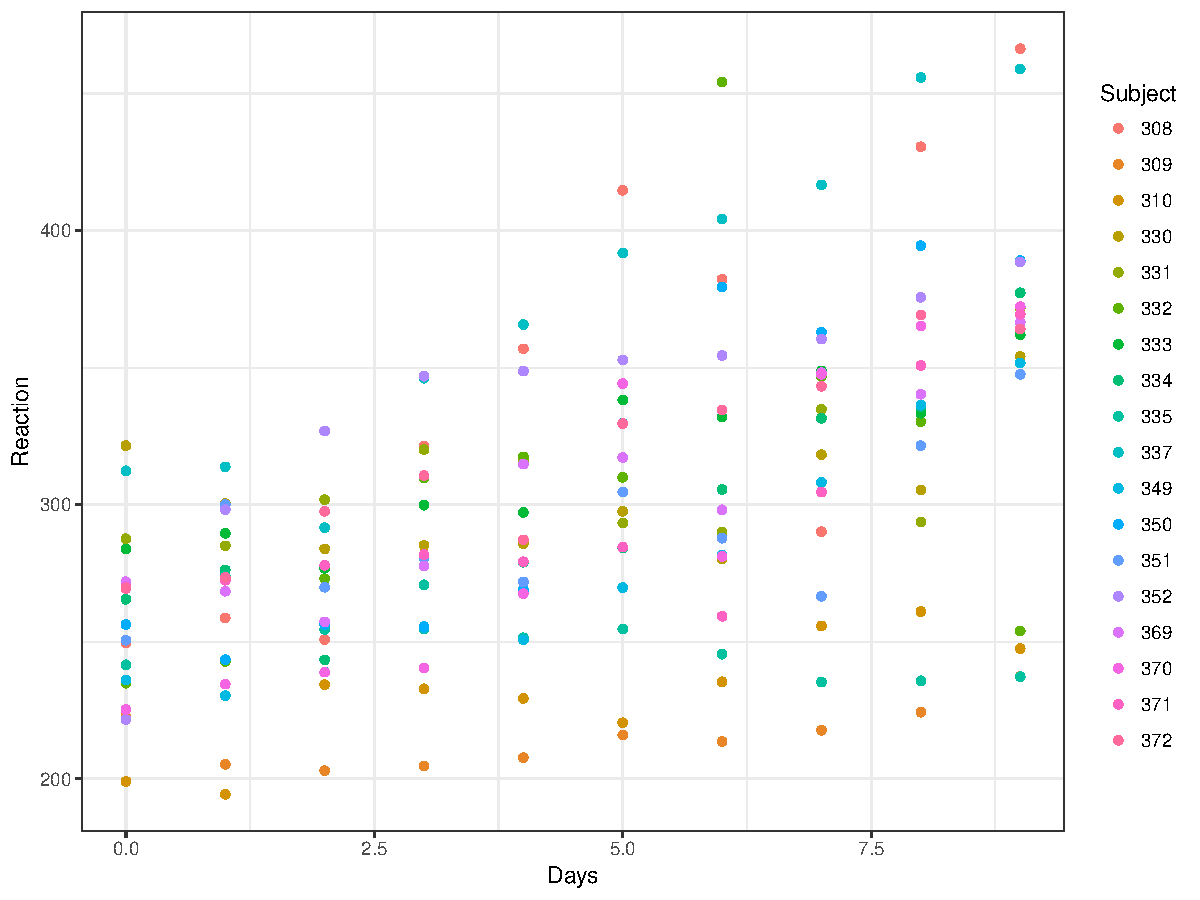
\includegraphics{Lec5_files/figure-beamer/unnamed-chunk-2-1.pdf}

\end{frame}

\begin{frame}{EDA (small multiples)}

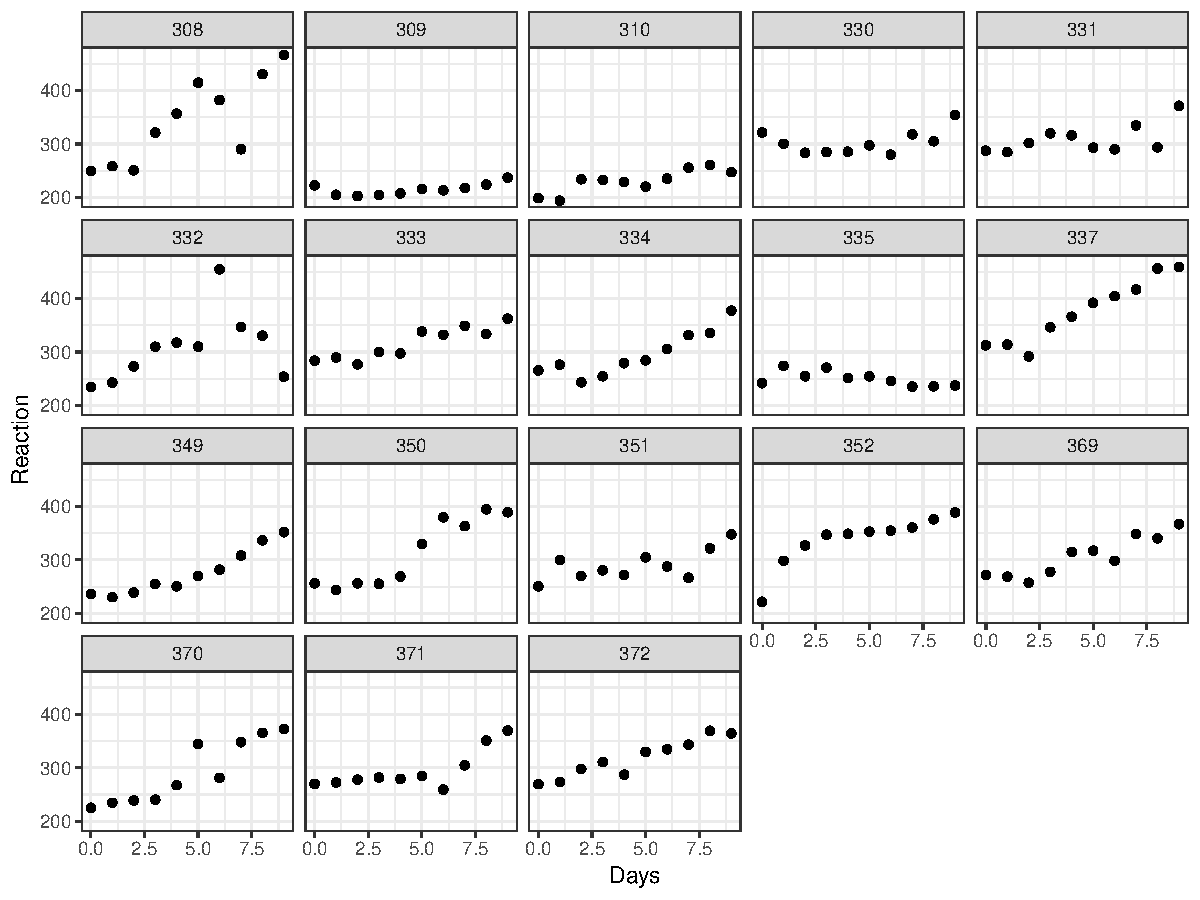
\includegraphics{Lec5_files/figure-beamer/unnamed-chunk-3-1.pdf}

\end{frame}

\begin{frame}[fragile]{Bayesian Linear Model}

\begin{verbatim}
## model{
##   # Likelihood
##   for(i in 1:length(Reaction)){
##     Reaction[i] ~ dnorm(mu[i],tau2)
##     mu[i] <- beta_0 + beta_1*Days[i]
## 
##     Y_hat[i] ~ dnorm(mu[i],tau2)
##   }
## 
##   # Prior for beta
##   beta_0 ~ dnorm(0,1/10000)
##   beta_1 ~ dnorm(0,1/10000)
## 
##   # Prior for sigma / tau2
##   sigma ~ dunif(0, 100) 
##   tau2 <- 1/(sigma*sigma)
## }
\end{verbatim}

\end{frame}

\begin{frame}{MCMC Diagnostics}

\begin{center}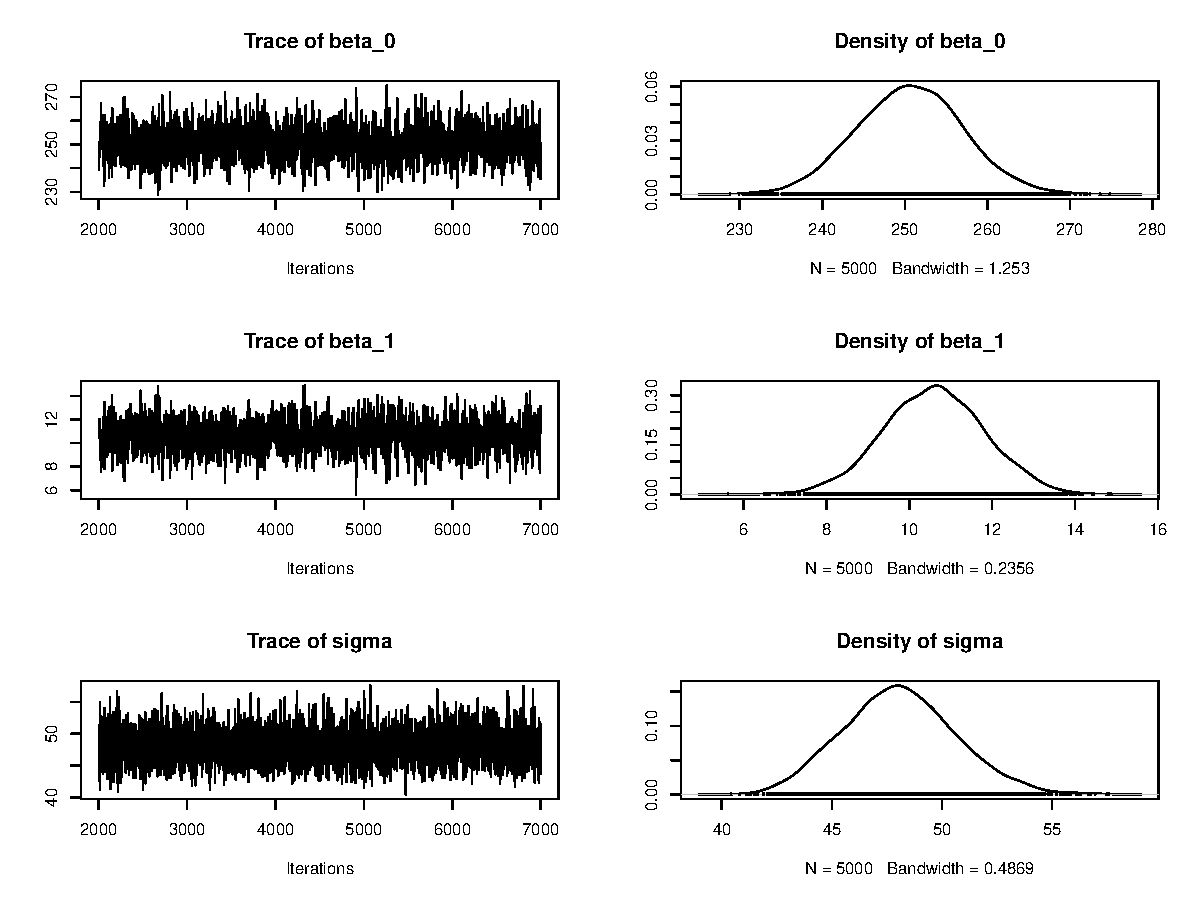
\includegraphics{Lec5_files/figure-beamer/unnamed-chunk-6-1} \end{center}

\end{frame}

\begin{frame}{Model fit}

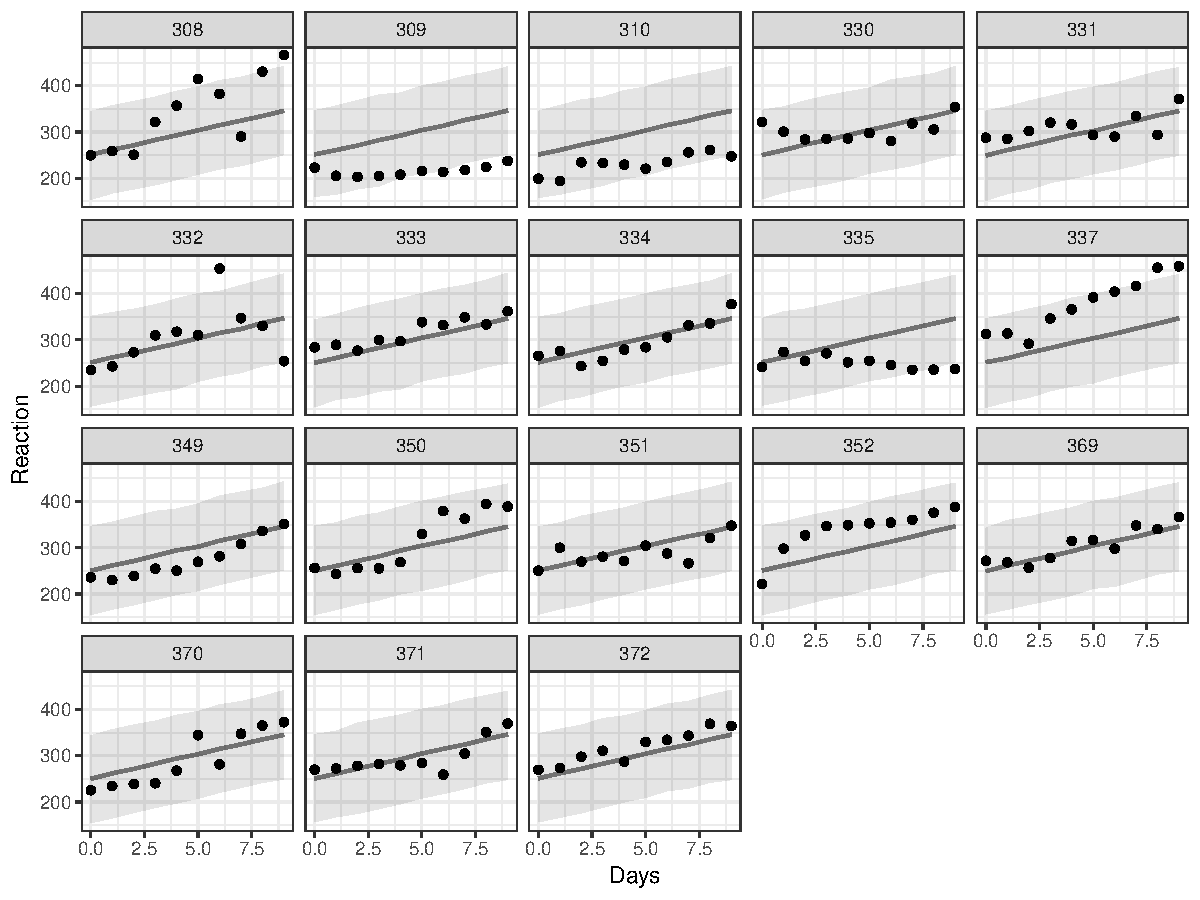
\includegraphics{Lec5_files/figure-beamer/unnamed-chunk-8-1.pdf}

\end{frame}

\begin{frame}{Residuals}

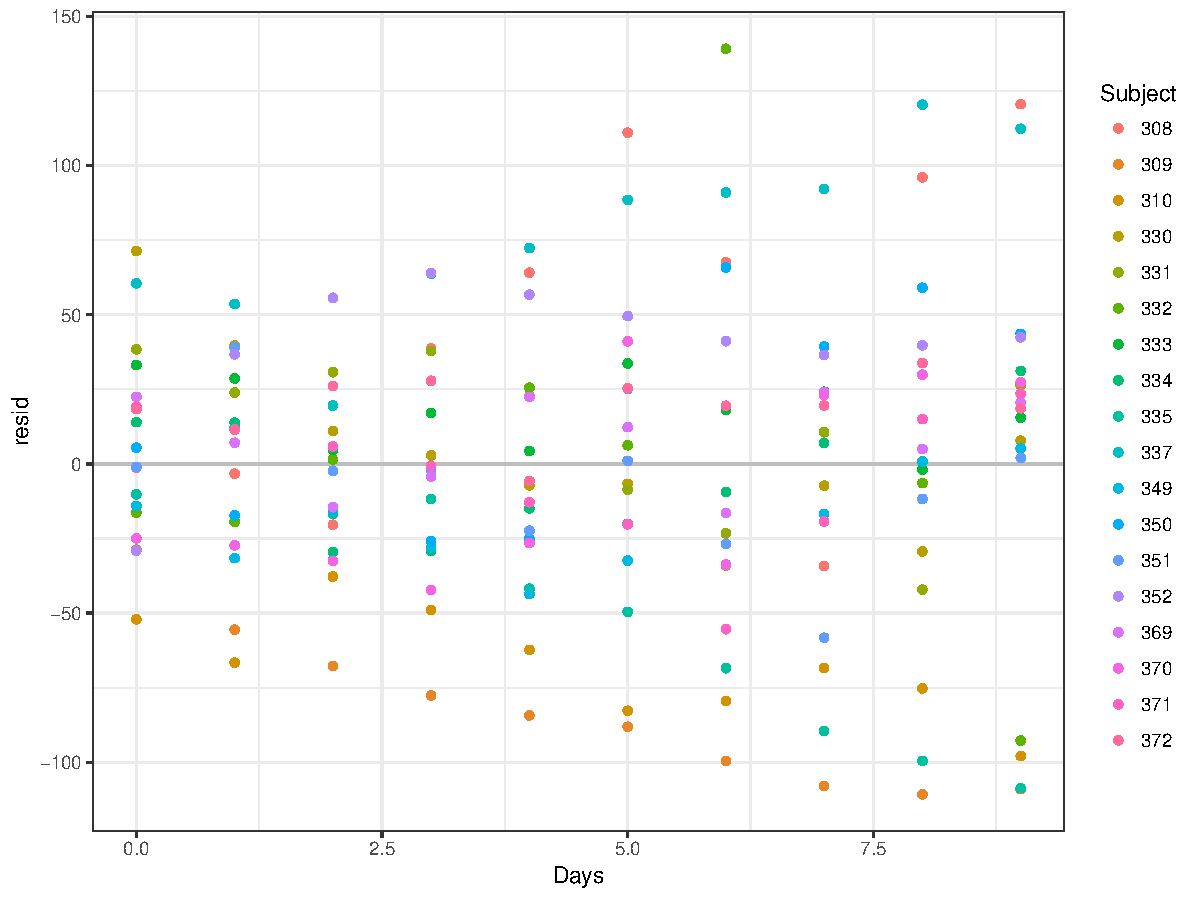
\includegraphics{Lec5_files/figure-beamer/unnamed-chunk-9-1.pdf}

\end{frame}

\begin{frame}{Residuals by subject}

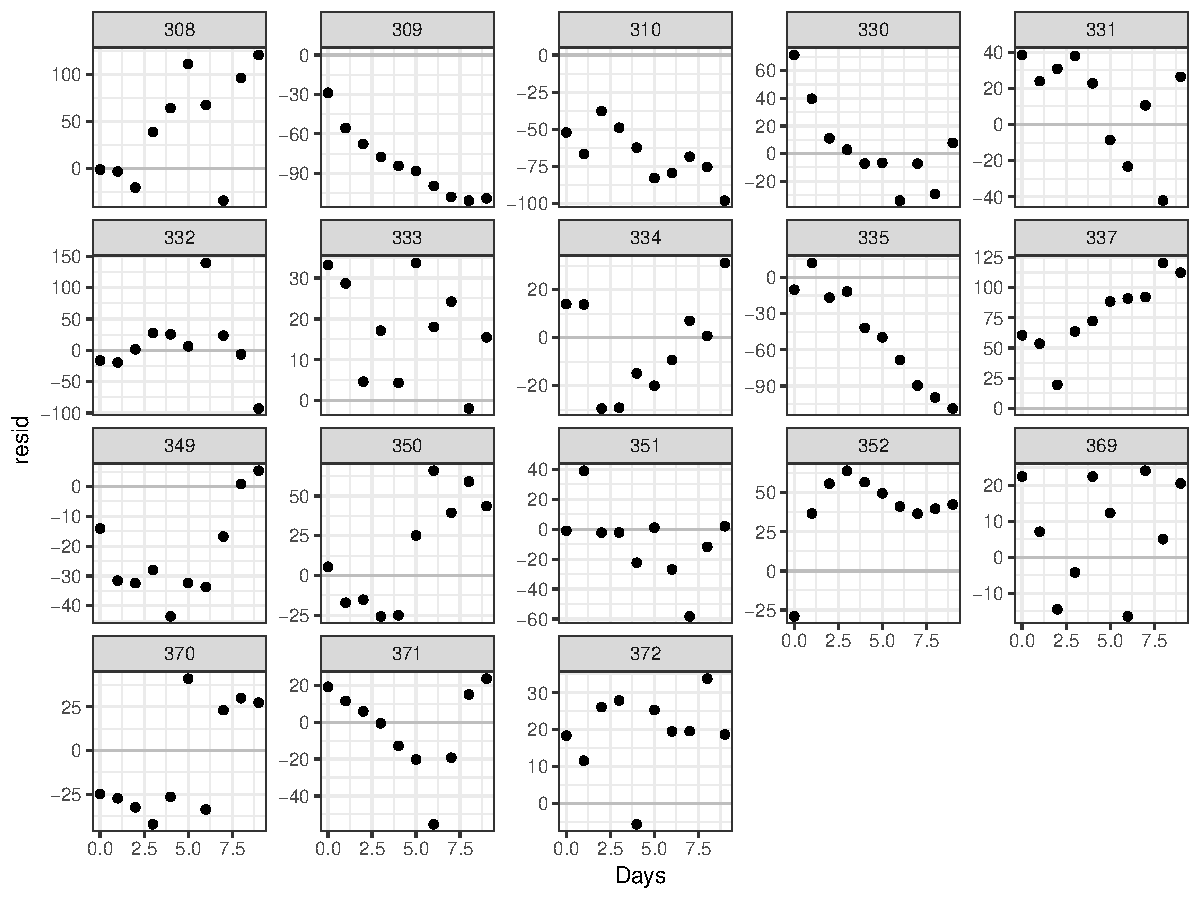
\includegraphics{Lec5_files/figure-beamer/unnamed-chunk-10-1.pdf}

\end{frame}

\section{Random Intercept Model}\label{random-intercept-model}

\begin{frame}[fragile]{Data coding}

\begin{Shaded}
\begin{Highlighting}[]
\NormalTok{sleepstudy =}\StringTok{ }\NormalTok{sleepstudy }\OperatorTok\StringTok{ }
\StringTok{  }\KeywordTok{mutate}\NormalTok{(}\DataTypeTok{Subject_index =} \KeywordTok{as.integer}\NormalTok{(Subject))}

\NormalTok{sleepstudy[}\KeywordTok{c}\NormalTok{(}\DecValTok{1}\OperatorTok{:}\DecValTok{2}\NormalTok{,}\DecValTok{11}\OperatorTok{:}\DecValTok{12}\NormalTok{,}\DecValTok{21}\OperatorTok{:}\DecValTok{22}\NormalTok{,}\DecValTok{31}\OperatorTok{:}\DecValTok{32}\NormalTok{),]}
\NormalTok{##    Reaction Days Subject Subject_index}
\NormalTok{## 1  249.5600    0     308             1}
\NormalTok{## 2  258.7047    1     308             1}
\NormalTok{## 11 222.7339    0     309             2}
\NormalTok{## 12 205.2658    1     309             2}
\NormalTok{## 21 199.0539    0     310             3}
\NormalTok{## 22 194.3322    1     310             3}
\NormalTok{## 31 321.5426    0     330             4}
\NormalTok{## 32 300.4002    1     330             4}
\end{Highlighting}
\end{Shaded}

\end{frame}

\begin{frame}{Random Intercept Model}

Let \(i\) represent each observation and \(j(i)\) be subject in
oberservation \(i\) then

\[ Y_i = \alpha_{j(i)}+ \beta_1 \times \text{Days} + \epsilon_i \]

\[
\begin{aligned}
\alpha_j &\sim \mathcal{N}(\beta_0,~\sigma^2_\alpha)  \\
\epsilon_i &\sim \mathcal{N}(0,~\sigma^2) \\
\\
\beta_0, \beta_1 &\sim \mathcal{N}(0, 10000)\\
\sigma, \sigma_\alpha &\sim \text{Unif}(0,100)
\end{aligned}
\]

\end{frame}

\begin{frame}[fragile]{Random Intercept Model - JAGS}

\begin{verbatim}
## model{
##   for(i in 1:length(Reaction)) {
##     Reaction[i] ~ dnorm(mu[i],tau2)
##     mu[i] <- alpha[Subject_index[i]] + beta_1*Days[i]
## 
##     Y_hat[i] ~ dnorm(mu[i],tau2)
##   }
## 
##   for(j in 1:18) {
##     alpha[j] ~ dnorm(beta_0, tau2_alpha)
##   }
##   
##   sigma_alpha ~ dunif(0, 100) 
##   tau2_alpha <- 1/(sigma_alpha*sigma_alpha)
## 
##   beta_0 ~ dnorm(0,1/10000)
##   beta_1 ~ dnorm(0,1/10000)
## 
##   sigma ~ dunif(0, 100) 
##   tau2 <- 1/(sigma*sigma)
## }
\end{verbatim}

\end{frame}

\begin{frame}{MCMC Diagnostics}

\begin{center}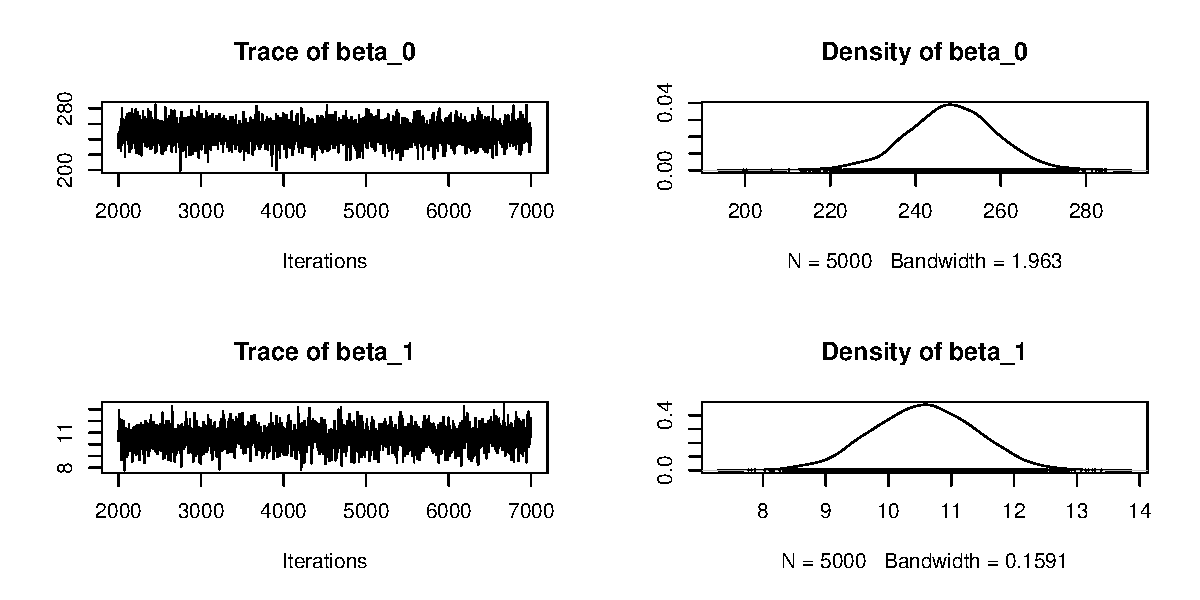
\includegraphics{Lec5_files/figure-beamer/unnamed-chunk-14-1} \end{center}

\end{frame}

\begin{frame}{}

\begin{center}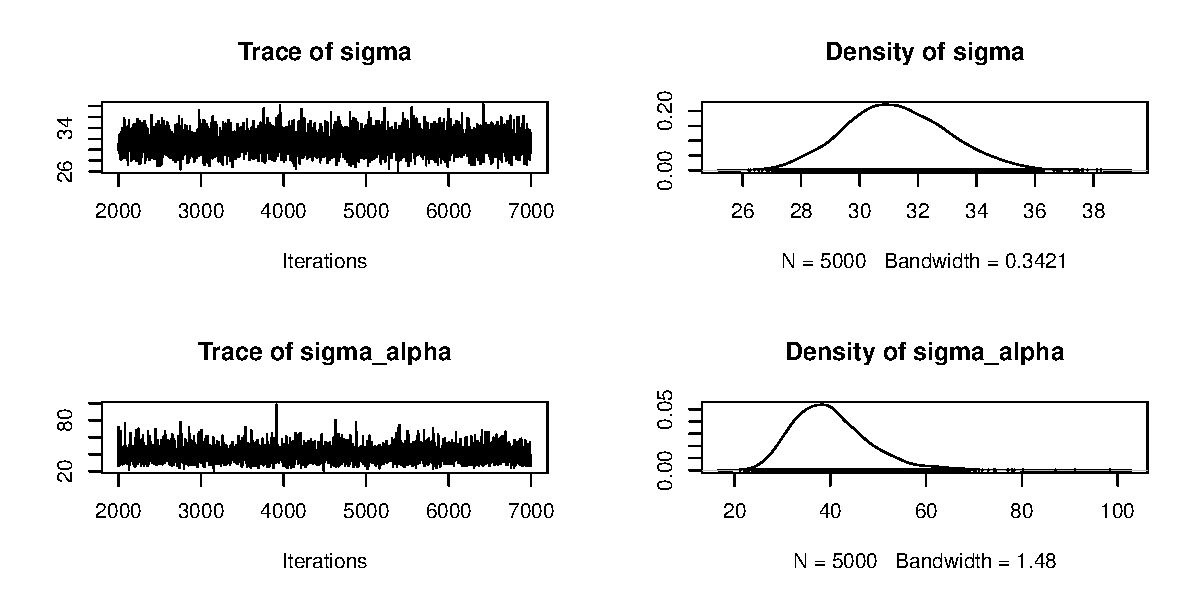
\includegraphics{Lec5_files/figure-beamer/unnamed-chunk-15-1} \end{center}

\end{frame}

\begin{frame}{}

\begin{center}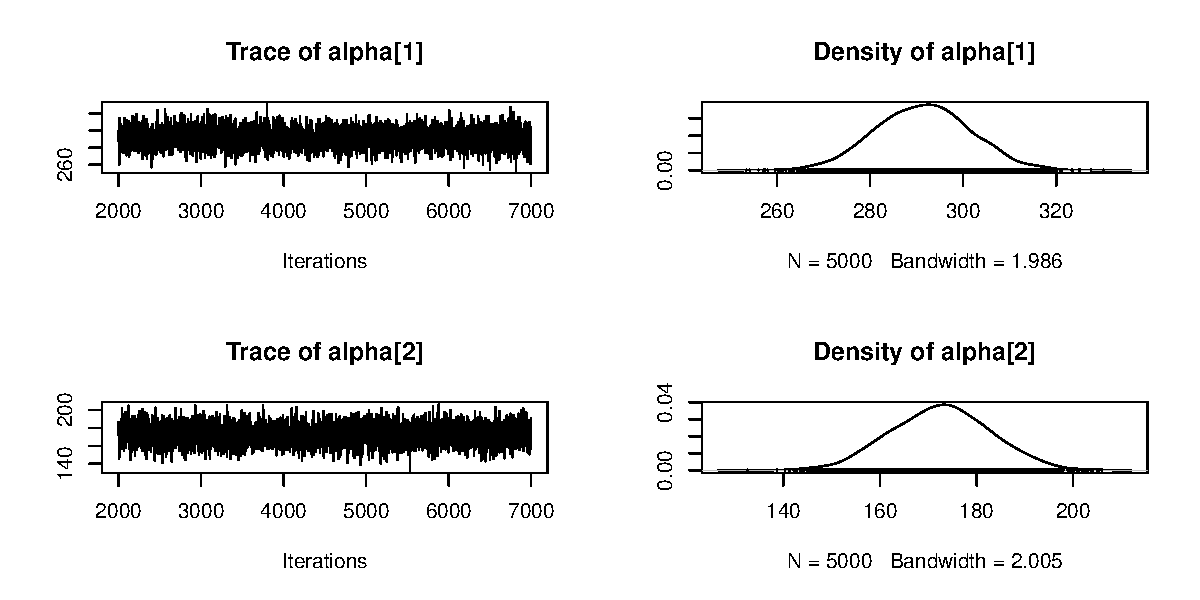
\includegraphics{Lec5_files/figure-beamer/unnamed-chunk-16-1} \end{center}

\end{frame}

\begin{frame}{Model fit}

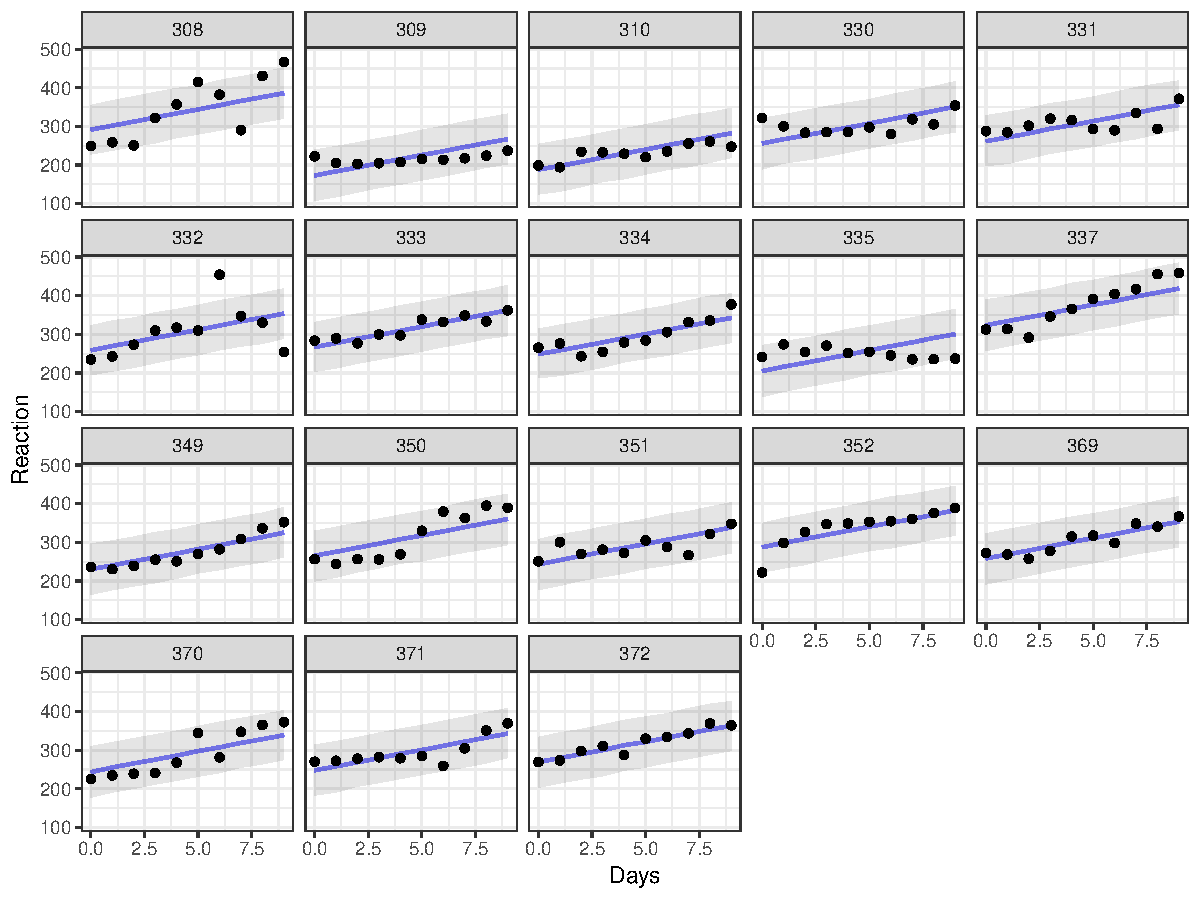
\includegraphics{Lec5_files/figure-beamer/unnamed-chunk-18-1.pdf}

\end{frame}

\begin{frame}{Residuals by subject}

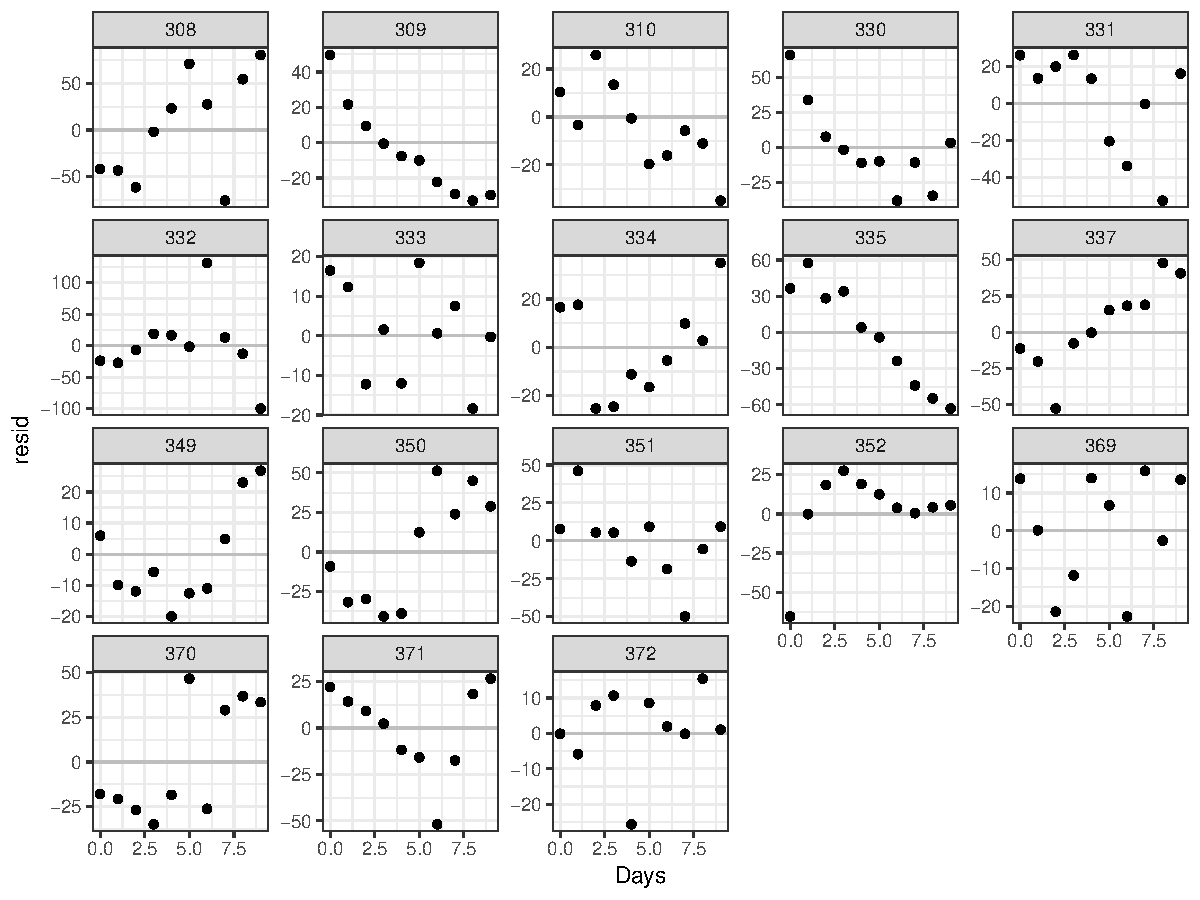
\includegraphics{Lec5_files/figure-beamer/unnamed-chunk-19-1.pdf}

\end{frame}

\begin{frame}{Random effects}

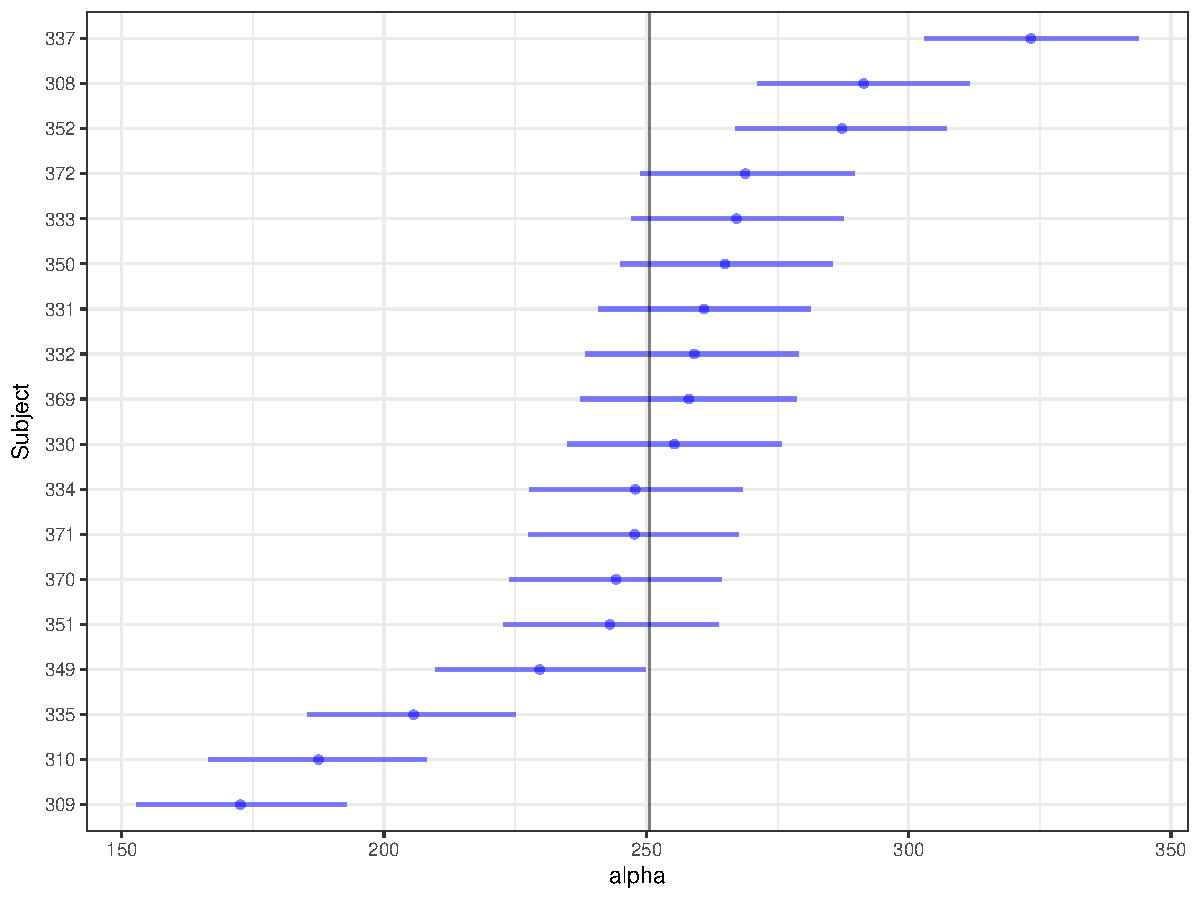
\includegraphics{Lec5_files/figure-beamer/unnamed-chunk-20-1.pdf}

\end{frame}

\begin{frame}[fragile]{Why not a fixed effect for Subject?}

\small

Not going to bother with the Bayesian model here because of all the
dummy coding and betas \ldots{} . . .

\begin{Shaded}
\begin{Highlighting}[]
\NormalTok{l =}\StringTok{ }\KeywordTok{lm}\NormalTok{(Reaction }\OperatorTok{~}\StringTok{ }\NormalTok{Days }\OperatorTok{+}\StringTok{ }\NormalTok{Subject }\OperatorTok{-}\StringTok{ }\DecValTok{1}\NormalTok{, }\DataTypeTok{data=}\NormalTok{sleepstudy)}
\KeywordTok{summary}\NormalTok{(l)}
\NormalTok{## }
\NormalTok{## Call:}
\NormalTok{## lm(formula = Reaction ~ Days + Subject - 1, data = sleepstudy)}
\NormalTok{## }
\NormalTok{## Residuals:}
\NormalTok{##      Min       1Q   Median       3Q      Max }
\NormalTok{## -100.540  -16.389   -0.341   15.215  131.159 }
\NormalTok{## }
\NormalTok{## Coefficients:}
\NormalTok{##            Estimate Std. Error t value Pr(>|t|)    }
\NormalTok{## Days        10.4673     0.8042   13.02   <2e-16 ***}
\NormalTok{## Subject308 295.0310    10.4471   28.24   <2e-16 ***}
\NormalTok{## Subject309 168.1302    10.4471   16.09   <2e-16 ***}
\NormalTok{## Subject310 183.8985    10.4471   17.60   <2e-16 ***}
\NormalTok{## Subject330 256.1186    10.4471   24.52   <2e-16 ***}
\NormalTok{## Subject331 262.3333    10.4471   25.11   <2e-16 ***}
\NormalTok{## Subject332 260.1993    10.4471   24.91   <2e-16 ***}
\NormalTok{## Subject333 269.0555    10.4471   25.75   <2e-16 ***}
\NormalTok{## Subject334 248.1993    10.4471   23.76   <2e-16 ***}
\NormalTok{## Subject335 202.9673    10.4471   19.43   <2e-16 ***}
\NormalTok{## Subject337 328.6182    10.4471   31.45   <2e-16 ***}
\NormalTok{## Subject349 228.7317    10.4471   21.89   <2e-16 ***}
\NormalTok{## Subject350 266.4999    10.4471   25.51   <2e-16 ***}
\NormalTok{## Subject351 242.9950    10.4471   23.26   <2e-16 ***}
\NormalTok{## Subject352 290.3188    10.4471   27.79   <2e-16 ***}
\NormalTok{## Subject369 258.9319    10.4471   24.79   <2e-16 ***}
\NormalTok{## Subject370 244.5990    10.4471   23.41   <2e-16 ***}
\NormalTok{## Subject371 247.8813    10.4471   23.73   <2e-16 ***}
\NormalTok{## Subject372 270.7833    10.4471   25.92   <2e-16 ***}
\NormalTok{## ---}
\NormalTok{## Signif. codes:  0 '***' 0.001 '**' 0.01 '*' 0.05 '.' 0.1 ' ' 1}
\NormalTok{## }
\NormalTok{## Residual standard error: 30.99 on 161 degrees of freedom}
\NormalTok{## Multiple R-squared:  0.9907, Adjusted R-squared:  0.9896 }
\NormalTok{## F-statistic: 901.6 on 19 and 161 DF,  p-value: < 2.2e-16}
\end{Highlighting}
\end{Shaded}

\end{frame}

\begin{frame}{Comparing Model fit}

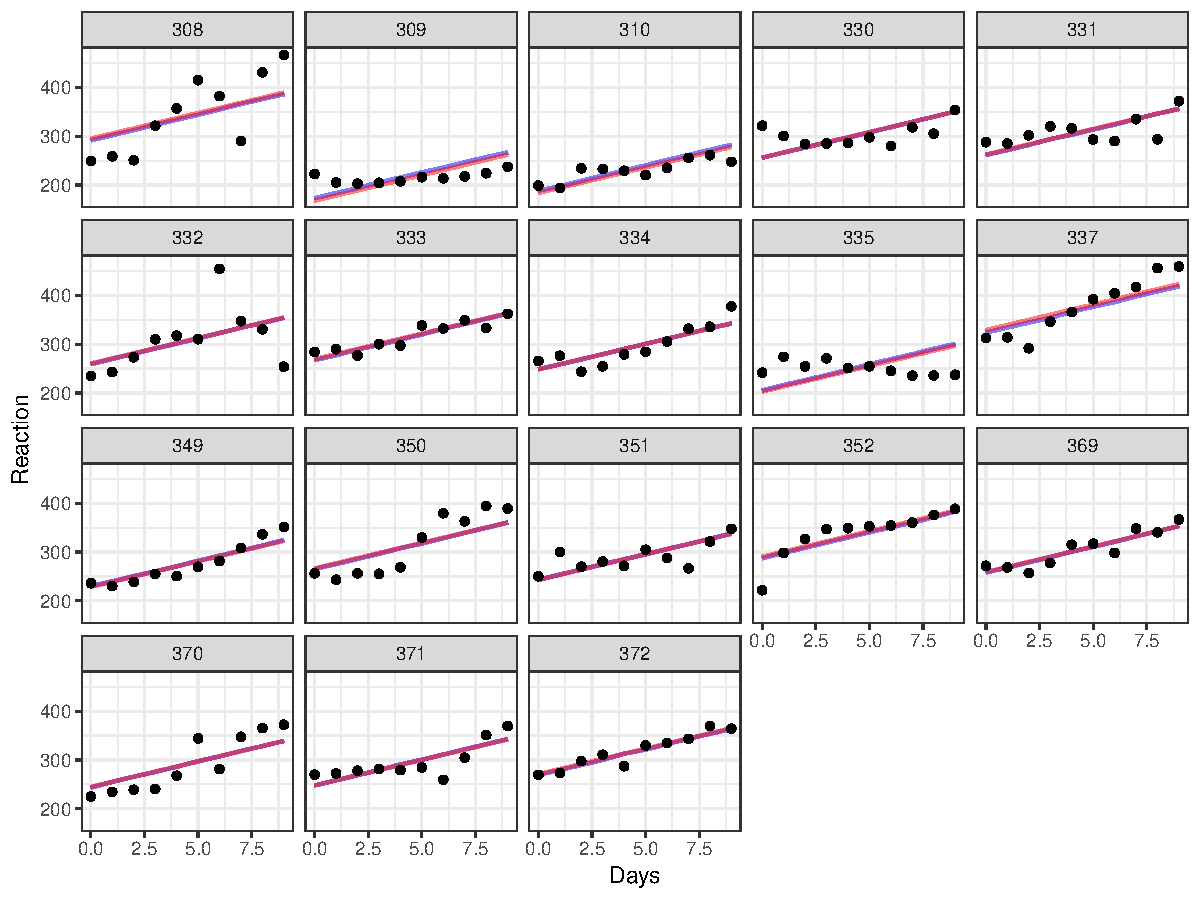
\includegraphics{Lec5_files/figure-beamer/unnamed-chunk-23-1.pdf}

\end{frame}

\begin{frame}{}

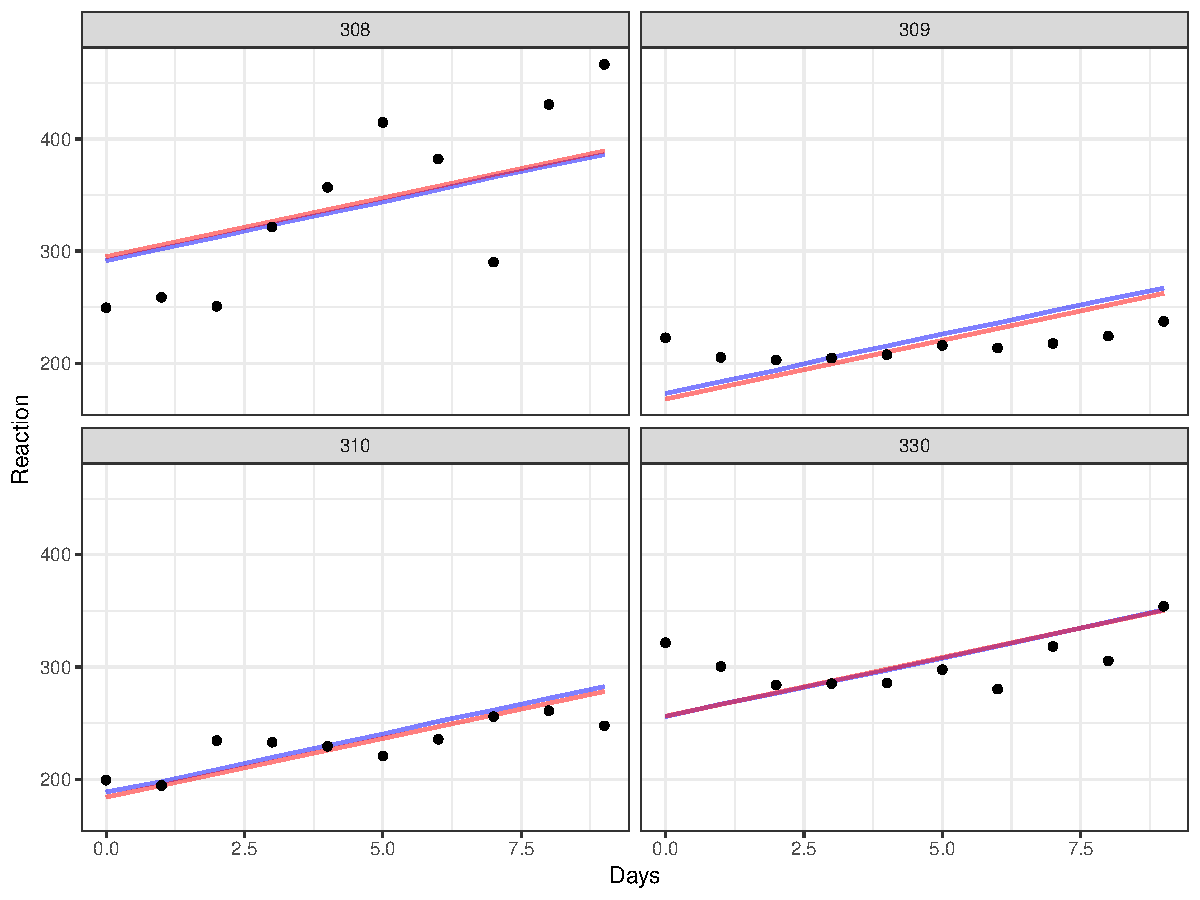
\includegraphics{Lec5_files/figure-beamer/unnamed-chunk-24-1.pdf}

\end{frame}

\begin{frame}{Random effects vs fixed effects}

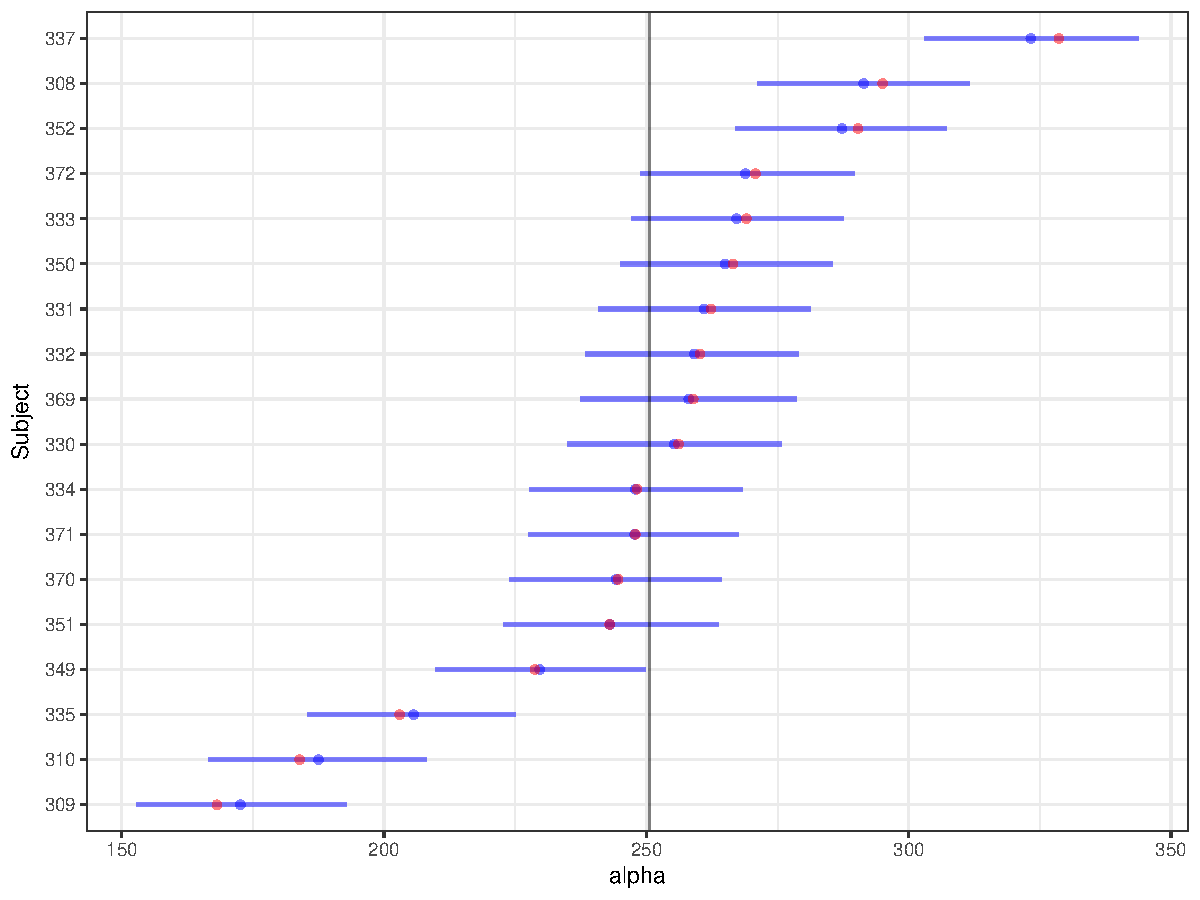
\includegraphics{Lec5_files/figure-beamer/unnamed-chunk-25-1.pdf}

\end{frame}

\begin{frame}[fragile]{Random Intercept Model (Informative prior for
\(\sigma_\alpha\))}

\begin{verbatim}
## model{
##   for(i in 1:length(Reaction)) {
##     Reaction[i] ~ dnorm(mu[i],tau2)
##     mu[i] <- alpha[Subject_index[i]] + beta_1*Days[i]
## 
##     Y_hat[i] ~ dnorm(mu[i],tau2)
##   }
## 
##   for(j in 1:18) {
##     alpha[j] ~ dnorm(beta_0, tau2_alpha)
##   }
##   
##   sigma_alpha ~ dunif(0, 10) 
##   tau2_alpha <- 1/(sigma_alpha*sigma_alpha)
## 
##   beta_0 ~ dnorm(0,1/10000)
##   beta_1 ~ dnorm(0,1/10000)
## 
##   sigma ~ dunif(0, 100) 
##   tau2 <- 1/(sigma*sigma)
## }
\end{verbatim}

\end{frame}

\begin{frame}{Comparing Model fit (Constrainged \(\alpha\))}

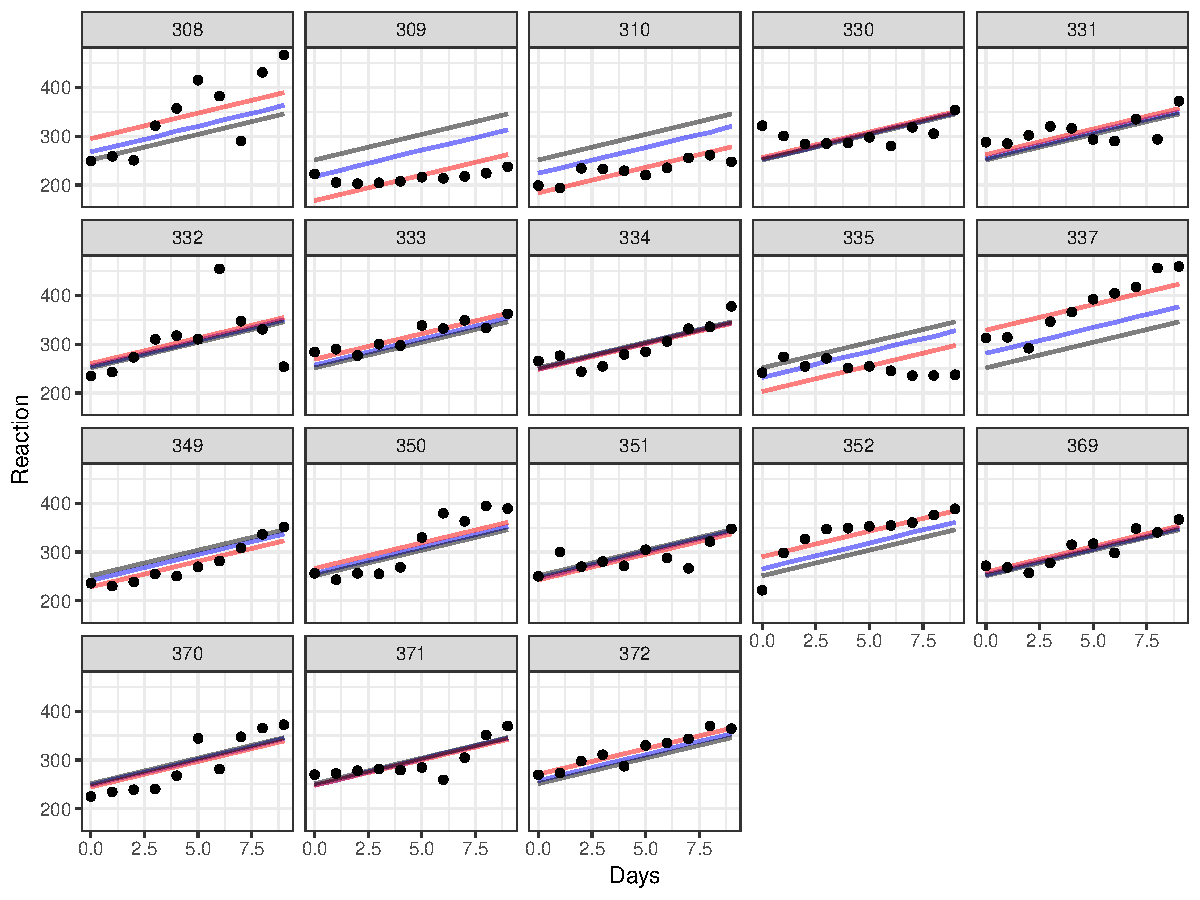
\includegraphics{Lec5_files/figure-beamer/unnamed-chunk-28-1.pdf}

\end{frame}

\begin{frame}{}

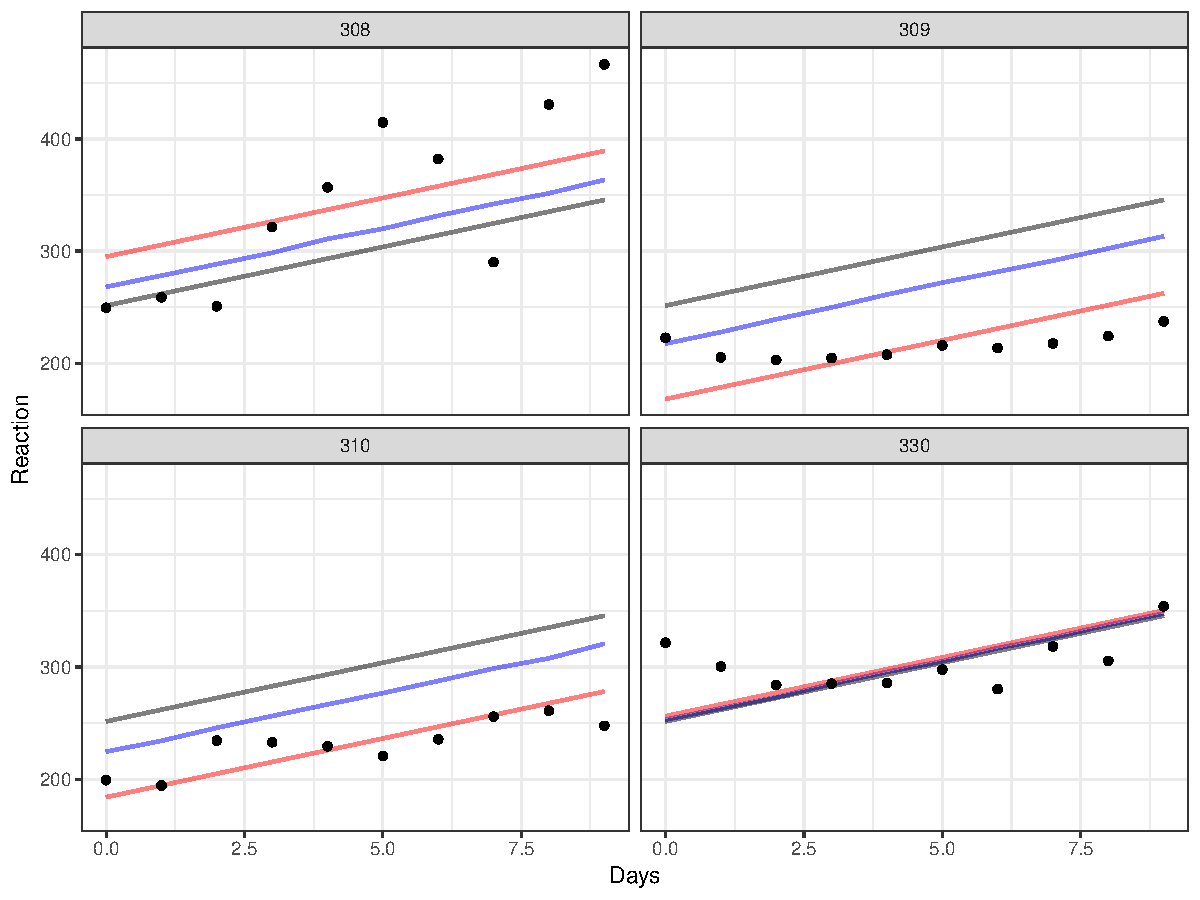
\includegraphics{Lec5_files/figure-beamer/unnamed-chunk-29-1.pdf}

\end{frame}

\begin{frame}{Prior Effect on \(\alpha\)}

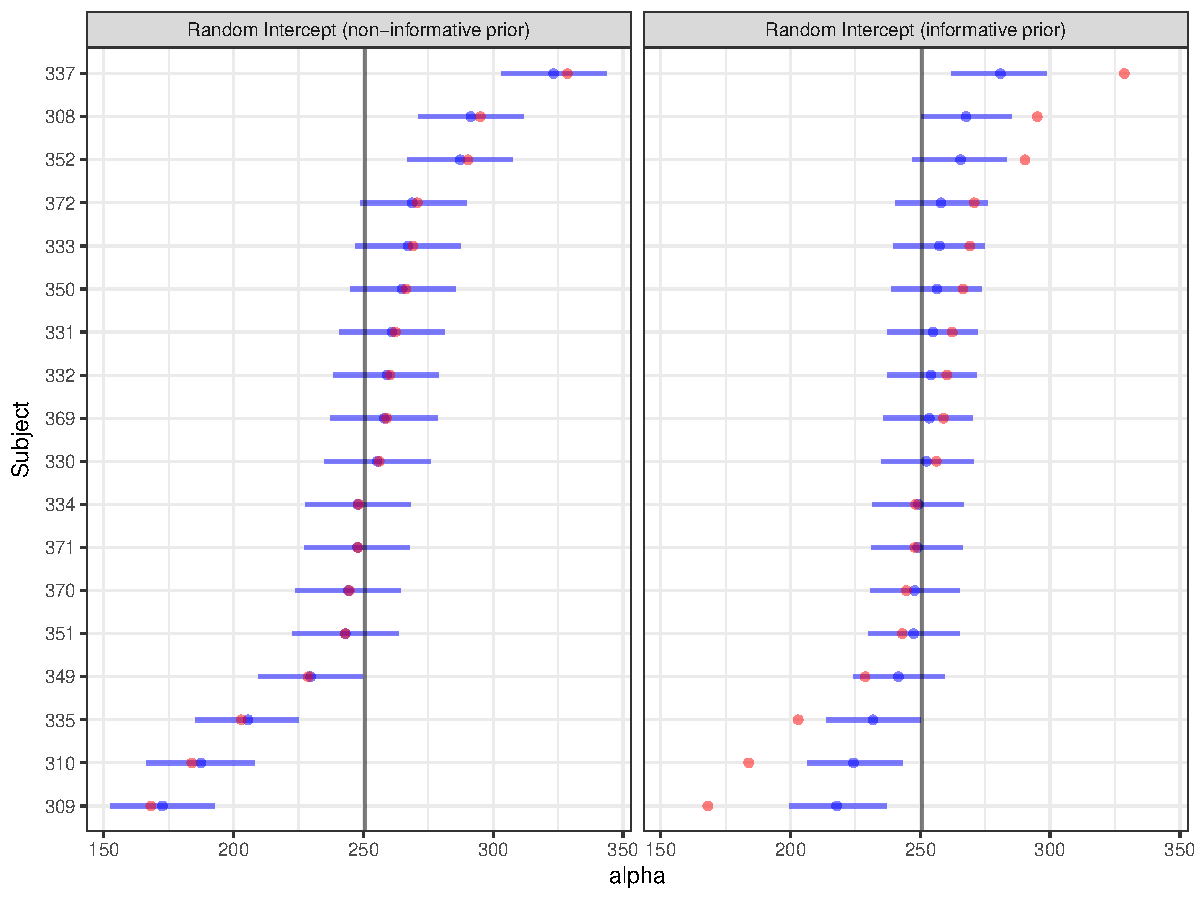
\includegraphics{Lec5_files/figure-beamer/unnamed-chunk-30-1.pdf}

\end{frame}

\begin{frame}{Some Distribution Theory (about
\(\bm{Y} ~|~ \beta_0, \beta_1, \sigma, \sigma_\alpha\))}

\end{frame}

\section{Random intercept and slope
model}\label{random-intercept-and-slope-model}

\begin{frame}{Model}

Let \(i\) represent each observation and \(j(i)\) be the subject in
oberservation \(i\) then

\[ Y_i = \alpha_{j(i)}+ \beta_{j(i)} \times \text{Days} + \epsilon_i \]

\[
\begin{aligned}
\alpha_j &\sim \mathcal{N}(\beta_0,~\sigma^2_\alpha)  \\
\beta_j &\sim \mathcal{N}(\beta_1,~\sigma^2_\beta) \\
\epsilon_i &\sim \mathcal{N}(0,~\sigma^2) \\
\\
\beta_0, \beta_1 &\sim \mathcal{N}(0, 10000)\\
\sigma, \sigma_\alpha, \sigma_\beta &\sim \text{Unif}(0,100)
\end{aligned}
\]

\end{frame}

\begin{frame}[fragile]{Model - JAGS}

\vspace{-2mm}

\begin{verbatim}
## model{
##   for(i in 1:length(Reaction)) {
##     Reaction[i] ~ dnorm(mu[i],tau2)
##     mu[i] <- alpha[Subject_index[i]] + beta[Subject_index[i]]*Days[i]
##     Y_hat[i] ~ dnorm(mu[i],tau2)
##   }
## 
##   sigma ~ dunif(0, 100) 
##   tau2 <- 1/(sigma*sigma)
## 
##   for(j in 1:18) {
##     alpha[j] ~ dnorm(beta_0, tau2_alpha)
##     beta[j]  ~ dnorm(beta_1, tau2_beta)
##   }
## 
##   beta_0 ~ dnorm(0,1/10000)
##   beta_1 ~ dnorm(0,1/10000)  
## 
##   sigma_alpha ~ dunif(0, 100) 
##   tau2_alpha <- 1/(sigma_alpha*sigma_alpha)
## 
##   sigma_beta ~ dunif(0, 100) 
##   tau2_beta <- 1/(sigma_beta*sigma_beta)
## }
\end{verbatim}

\end{frame}

\begin{frame}{Model fit}

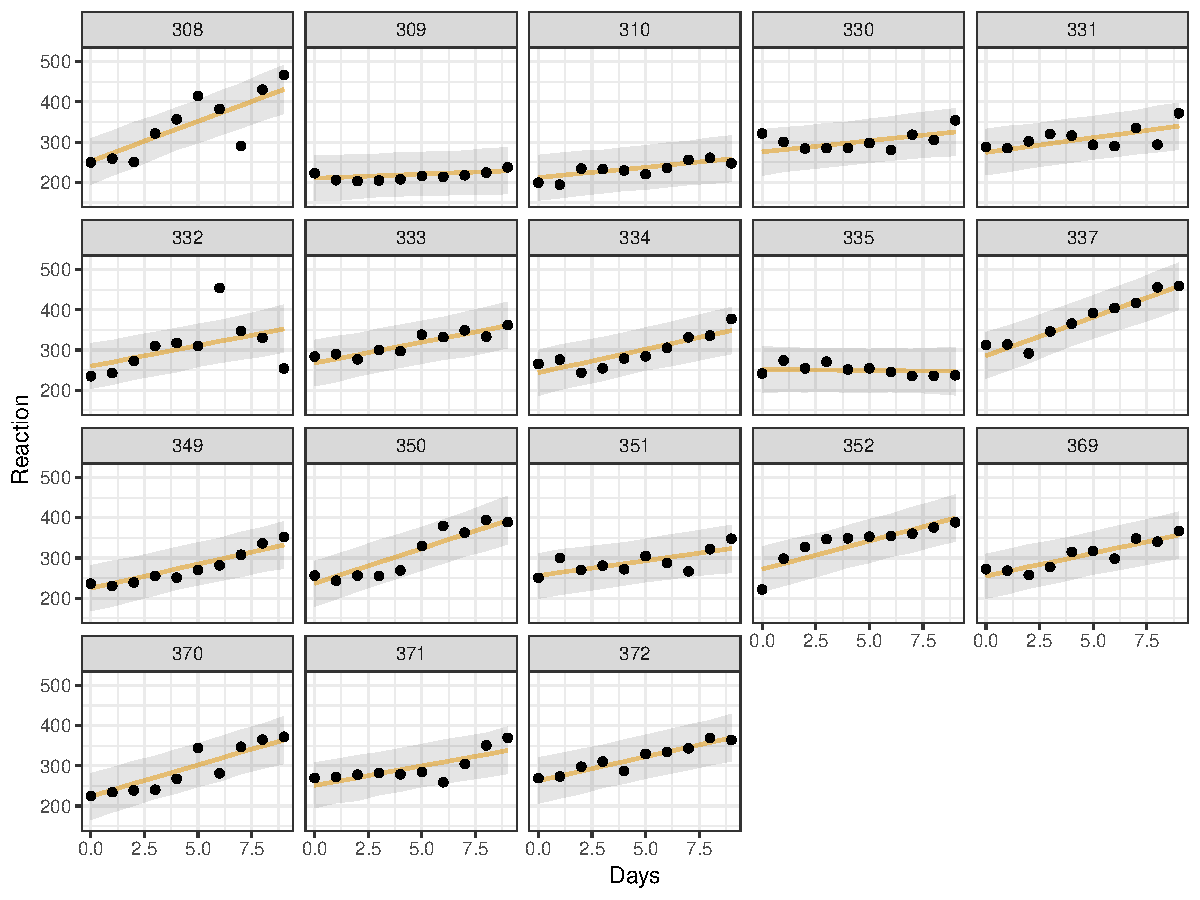
\includegraphics{Lec5_files/figure-beamer/unnamed-chunk-34-1.pdf}

\end{frame}

\begin{frame}{Comparison}

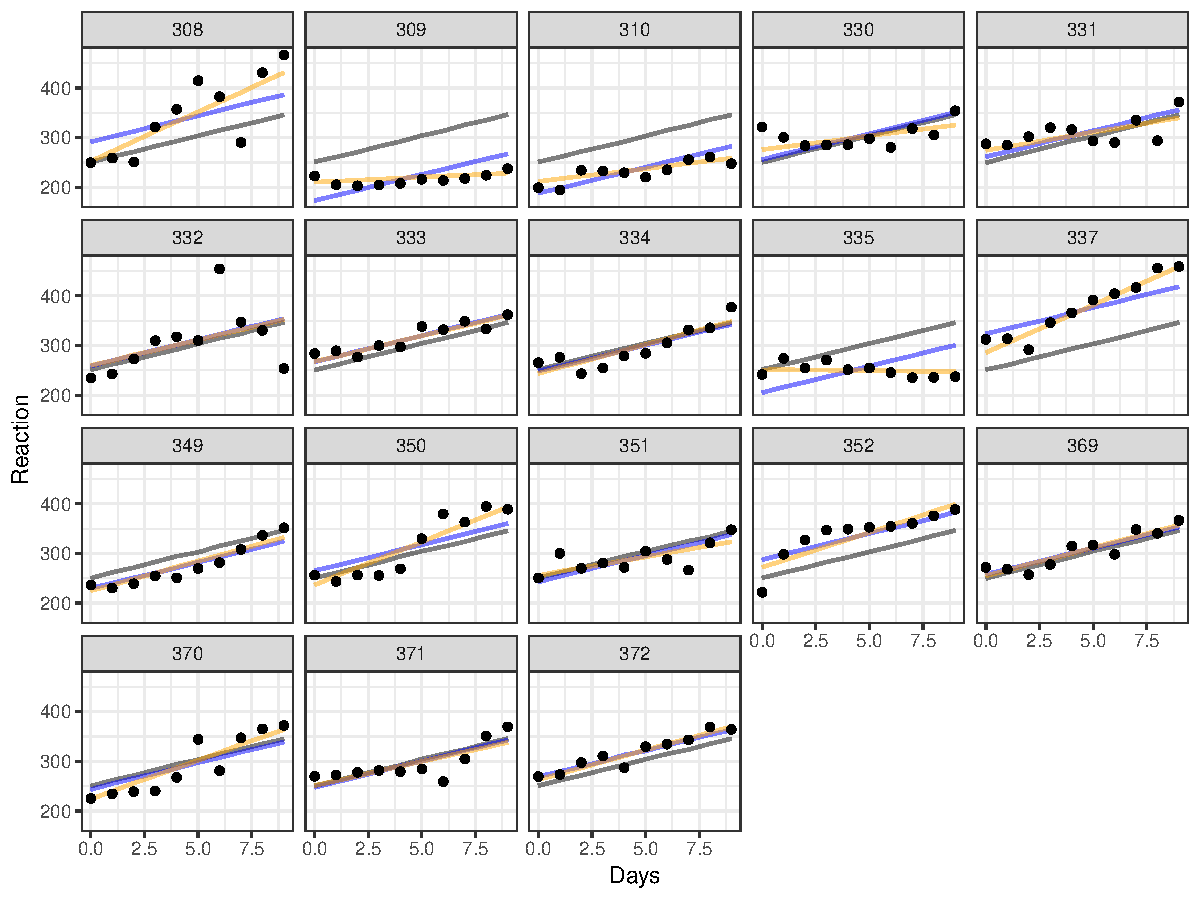
\includegraphics{Lec5_files/figure-beamer/unnamed-chunk-35-1.pdf}

\end{frame}

\begin{frame}{}

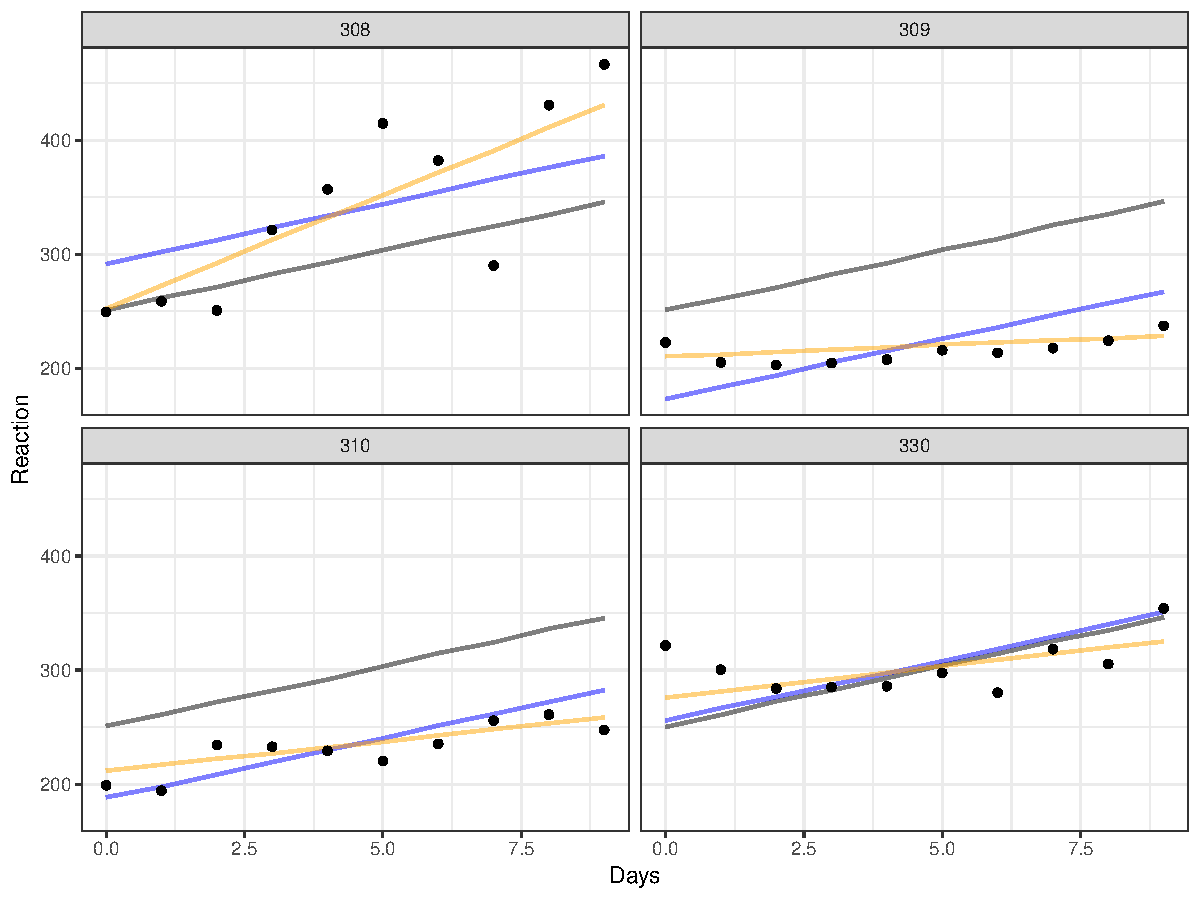
\includegraphics{Lec5_files/figure-beamer/unnamed-chunk-36-1.pdf}

\end{frame}

\begin{frame}{Residuals by subject}

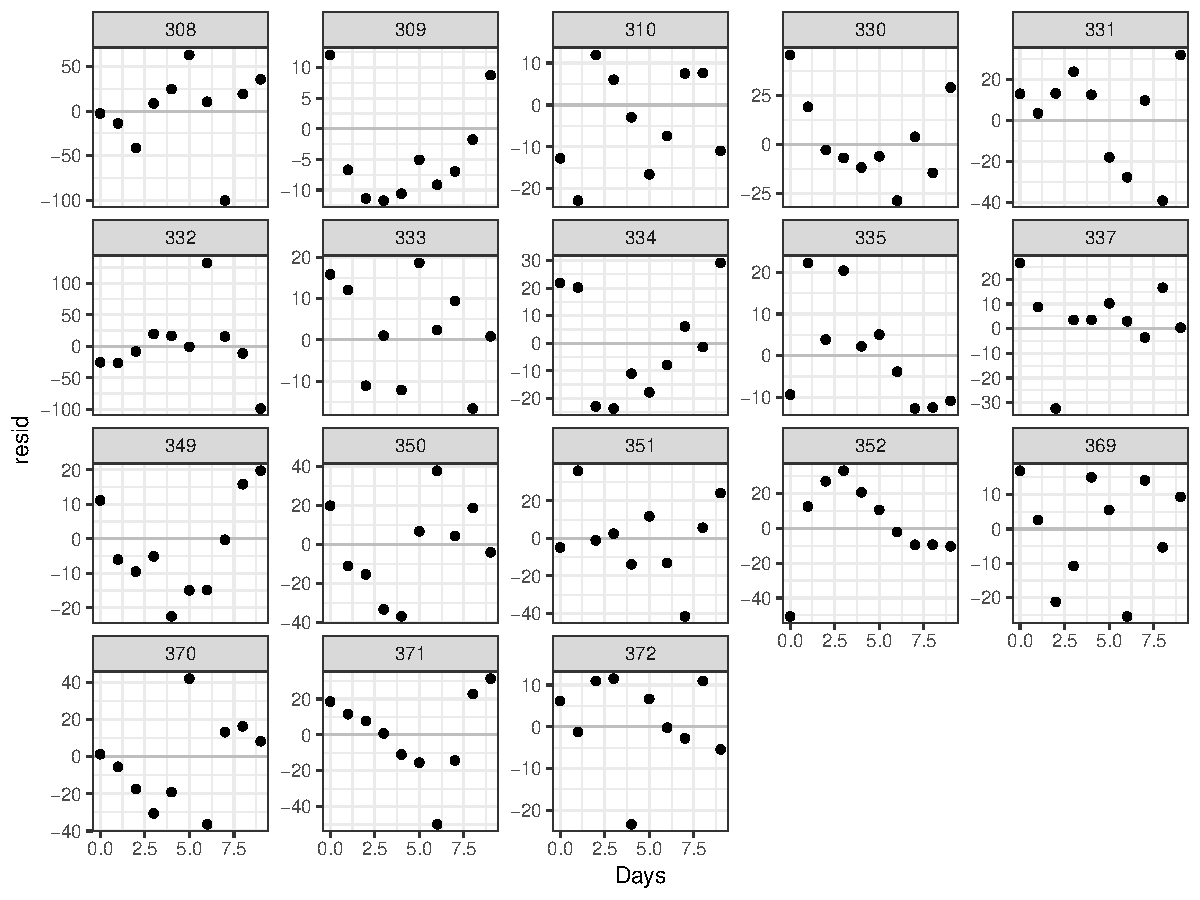
\includegraphics{Lec5_files/figure-beamer/unnamed-chunk-37-1.pdf}

\end{frame}

\end{document}
